\documentclass[11pt,a4paper]{article}

\usepackage[margin=2.2cm]{geometry}
\usepackage[T1]{fontenc}
\usepackage{lmodern}
\usepackage{microtype}
\usepackage{amsmath,amssymb}
\usepackage{graphicx}
\usepackage{booktabs}
\usepackage{tabularx}
\usepackage{multirow}
\usepackage{array}
\usepackage{xcolor}
\usepackage{float}
\usepackage[font=small,labelfont=bf]{caption}
\usepackage{algorithm}
\usepackage{algpseudocode}
\usepackage{enumitem}
\usepackage[colorlinks=true,linkcolor=blue!50!black,citecolor=blue!50!black,urlcolor=blue!50!black]{hyperref}

\graphicspath{{../results/figures/}}
\makeatletter\newcommand{\gen}[1]{\@@input generated/#1 }\makeatother
\setlist{nosep,leftmargin=*}
\setlength{\parskip}{3pt}

\title{\textbf{Parallel Conjugate Gradient for the 2D and 3D Poisson Equation\\ with MPI, MPI+OpenMP and MPI+CUDA}}
\author{
  DSA5208 Project 3 \quad AY2026/27 Semester 1 \quad National University of Singapore\\[6pt]
  \begin{tabular}{lll}
  Yikun Zhao & A0353894M & serial and MPI solvers, validation, report\\
  Jiahao Zhou & A0354090J & MPI+OpenMP and MPI+CUDA solvers\\
  Zheke Chen & A0356140M & cluster builds, experiments, analysis and figures
  \end{tabular}
}
\date{13 November 2026}

\begin{document}
\maketitle

\begin{abstract}
\noindent
We solve the Poisson equation $-\Delta u=f$ on the unit square and the unit cube with an
unpreconditioned, matrix-free conjugate gradient (CG) method and parallelise it in three ways:
pure MPI with a domain decomposition, hybrid MPI+OpenMP, and MPI+CUDA with one GPU per rank.
All versions share one CG driver and are validated against a manufactured solution (observed
second-order accuracy) and against the serial solver (identical iteration counts, pointwise
agreement to rounding error). On the Vanda cluster, pure MPI reaches $138\times$ speedup
on 256 cores for a 3D problem with $2.4\times10^{7}$ unknowns, but the 2D problem stops scaling
beyond one 64-core node because every CG iteration requires two global reductions whose
latency over the inter-node network ($\approx150$--$300~\mu$s each) exceeds the remaining
computation. Cartesian blocks beat 1D slabs by $5\times$ in 3D, a single-reduction CG variant
recovers up to 35\% at 256 cores, hybrid MPI+OpenMP does not beat pure MPI at fixed core count,
and one NVIDIA A40 GPU is about $19\times$ faster than one CPU core.
\end{abstract}

{\setcounter{tocdepth}{1}\small\tableofcontents}
\newpage

%=====================================================================
\section{Introduction and the algorithm}\label{sec:intro}
%=====================================================================

\subsection{Model problem and discretisation}
We solve
\begin{equation}
  -\Delta u = f \quad\text{in } \Omega=(0,1)^d,\qquad u=0 \quad\text{on }\partial\Omega,\qquad d\in\{2,3\}.
\end{equation}
The domain is covered by a uniform grid with $n$ interior points per side, spacing
$h=1/(n+1)$ and points $x_i=(i+1)h$, $i=0,\dots,n-1$. The standard second-order
finite-difference approximation of $-\Delta$ uses the 5-point stencil in 2D and the 7-point
stencil in 3D,
\begin{equation}\label{eq:stencil}
  (A\mathbf u)_{\mathbf i} = \frac{1}{h^2}\Big(2d\,u_{\mathbf i}-\sum_{k=1}^{d}\big(u_{\mathbf i+\mathbf e_k}+u_{\mathbf i-\mathbf e_k}\big)\Big),
\end{equation}
with boundary values set to zero. This gives a linear system $A\mathbf u=\mathbf b$ with
$N=n^d$ unknowns. $A$ is sparse (at most $2d+1$ non-zeros per row, in total
$\mathrm{nnz}(A)=(2d+1)n^d-2d\,n^{d-1}$), symmetric and positive definite (SPD), with condition
number $\kappa(A)=\mathcal O(h^{-2})=\mathcal O(n^2)$.

\subsection{The conjugate gradient method}
CG~\cite{hestenes1952} is the standard Krylov method for SPD systems. Starting from $\mathbf x_0=0$,
each iteration performs one matrix--vector product, two inner products and three vector
updates (Algorithm~\ref{alg:cg}). We stop when the relative residual
$\|\mathbf r_k\|_2/\|\mathbf b\|_2$ falls below a tolerance (the program default is $10^{-8}$; all timed experiments used $5\times10^{-9}$, see Section~\ref{sec:setup}).
Without a preconditioner the number of iterations grows like $\sqrt{\kappa}=\mathcal O(n)$;
we deliberately keep CG unpreconditioned so that every iteration has exactly the same
communication structure and the parallel overheads can be studied in isolation.

\begin{algorithm}[H]
\caption{Standard CG (``\texttt{std}''): two global reductions per iteration}\label{alg:cg}
\begin{algorithmic}[1]
\State $\mathbf x=0,\ \mathbf r=\mathbf b,\ \mathbf p=\mathbf r,\ \rho=\mathbf r^{\top}\mathbf r$
\For{$k=1,2,\dots$}
  \State $\mathbf q = A\mathbf p$ \Comment{stencil sweep; needs neighbour values (halo exchange)}
  \State $\alpha=\rho/(\mathbf p^{\top}\mathbf q)$ \Comment{global reduction \#1}
  \State $\mathbf x \gets \mathbf x+\alpha\mathbf p,\quad \mathbf r\gets\mathbf r-\alpha\mathbf q$
  \State $\rho_{\text{new}}=\mathbf r^{\top}\mathbf r$ \Comment{global reduction \#2}
  \If{$\sqrt{\rho_{\text{new}}}/\|\mathbf b\| < \text{tol}$} \textbf{stop} \EndIf
  \State $\mathbf p\gets\mathbf r+(\rho_{\text{new}}/\rho)\,\mathbf p,\quad \rho\gets\rho_{\text{new}}$
\EndFor
\end{algorithmic}
\end{algorithm}

We also implement the Chronopoulos--Gear variant~\cite{chronopoulos1989} (``\texttt{pipe}'' in
our code), which computes $\gamma=\mathbf r^{\top}\mathbf r$ and $\delta=(A\mathbf r)^{\top}\mathbf r$
together in \emph{one} reduction per iteration and updates the extra vector
$\mathbf s=A\mathbf p$ by recurrence ($\mathbf s\gets\mathbf w+\beta\mathbf s$ with $\mathbf w=A\mathbf r$).
It produces the same iterates in exact arithmetic, trades one global reduction for two extra
vector updates, and is the standard remedy when reduction latency dominates.

\subsection{Why this algorithm is not embarrassingly parallel}
The matrix is never stored (a \emph{matrix-free} method): $A\mathbf p$ is a stencil sweep
over the grid. When the grid is distributed, a point next to a sub-domain boundary needs
values owned by a neighbouring process, so every iteration requires a \emph{halo exchange}
(point-to-point communication). Each inner product needs contributions from all processes, so
every iteration also requires two \emph{global reductions} (\texttt{MPI\_Allreduce}) that act
as synchronisation points: no process can compute $\alpha$ or $\beta$ before all others have
finished their part. The serial dependency between consecutive iterations means the iterations
cannot be distributed; only the work \emph{within} an iteration can.

\subsection{Synthetic data}\label{sec:data}
All data are synthetic and generated on the fly by every process for the points it owns. We
use the manufactured solution
\begin{equation}
  u(\mathbf x)=\prod_{k=1}^{d} g(x_k),\qquad g(t)=t(1-t)e^{t},\qquad
  f=-\Delta u=\sum_{k=1}^{d} t_k(t_k+3)e^{t_k}\prod_{j\neq k} g(x_j)\Big|_{t=\mathbf x},
\end{equation}
which vanishes on $\partial\Omega$ and has non-zero fourth derivatives, so the discretisation
error is exactly computable and of size $\mathcal O(h^2)$. The right-hand side is
$\mathbf b_{\mathbf i}=f(\mathbf x_{\mathbf i})$. We deliberately did \emph{not} use the common
choice $u=\prod_k\sin(\pi x_k)$: its grid samples form an exact eigenvector of $A$, so CG
converges in a single iteration and any timing would be meaningless. With our choice CG needs
$\approx3.2n$ iterations in 2D and $\approx3.8n$ in 3D (Table~\ref{tab:serial}), as for a
generic right-hand side. Problem size is controlled only by $n$, which makes weak-scaling
meshes easy to construct.

\subsection{Terminology}
\begin{table}[H]
\centering\small
\begin{tabularx}{\linewidth}{>{\raggedright\arraybackslash}p{3.6cm}X}
\toprule
Term & Meaning in this report\\
\midrule
rank & One MPI process. Each rank is pinned to its own physical core (or cores, with OpenMP).\\
halo / ghost layer & One extra layer of grid points around a rank's block holding copies of the neighbours' boundary values.\\
slab / Cartesian decomposition & Split of the grid into 1D slabs along the slowest axis, or into 2D/3D blocks over all axes (\texttt{MPI\_Dims\_create}/\texttt{MPI\_Cart\_create}).\\
blocking / overlapped halo & \texttt{MPI\_Sendrecv} before the stencil, or non-blocking \texttt{MPI\_Isend/Irecv} with the interior stencil computed while messages are in flight.\\
\texttt{std} / \texttt{pipe} CG & Standard CG (2 reductions per iteration) / Chronopoulos--Gear single-reduction CG (1 reduction).\\
strong scaling & Fixed global problem, increasing core count $P$. Speedup $S(P)=T(1)/T(P)$, efficiency $E(P)=S(P)/P$, where $T(1)$ is the one-rank MPI run.\\
weak scaling & Fixed work per core ($N/P$ constant). Weak efficiency $E_w(P)=T(1)/T(P)$; per-iteration weak efficiency uses time per CG iteration.\\
superlinear speedup & $S(P)>P$, here caused by the working set fitting in cache once it is split over enough cores.\\
memory-bandwidth bound & Runtime limited by the rate at which data is moved from main memory, not by arithmetic.\\
true residual & $\|\mathbf b-A\mathbf x\|/\|\mathbf b\|$ recomputed after the solve, as opposed to the recursively updated $\|\mathbf r_k\|$.\\
CUDA-aware MPI (device transport) & MPI accepts GPU memory pointers directly. In the \emph{staged} transport the halo is copied to host memory first.\\
\texttt{MPI\_THREAD\_FUNNELED} & Thread-support level in which only the master thread makes MPI calls.\\
phase times & Per-rank accumulated time in the \emph{stencil} (stencil and vector updates), \emph{halo} (neighbour exchange) and \emph{reduce} (local dot product, \texttt{MPI\_Allreduce} and any wait for slower ranks) phases; we report the maximum over ranks.\\
\bottomrule
\end{tabularx}
\end{table}

%=====================================================================
\section{Implementation and parallelisation design}\label{sec:design}
%=====================================================================

\subsection{Software structure}
The CG algorithm (both variants) is written once, in \texttt{src/common/cg.cpp}, against an
abstract \texttt{Backend} interface: vector allocation, \texttt{apply} ($\mathbf q=A\mathbf p$,
including any halo exchange), global \texttt{dot} and fused \texttt{dot2}, and the vector updates
\texttt{axpy}/\texttt{xpay}. The serial, MPI and MPI+OpenMP solvers are three implementations of
this interface; MPI+OpenMP inherits the MPI backend and replaces only its compute loops. The CUDA
solver keeps its own CG loop on the device but uses the same problem definition, command-line
interface and output format. Consequently all CPU versions execute the identical sequence of
floating-point operations up to the order of summation, which is what makes the strict
serial-versus-parallel validation in Section~\ref{sec:validation} possible. No BLAS, LAPACK or other
linear-algebra library is used. Table~\ref{tab:techniques} summarises how each part of CG is
parallelised in each version.

\begin{table}[H]
\centering\small
\caption{How each part of one CG iteration is parallelised.}\label{tab:techniques}
\begin{tabularx}{\linewidth}{>{\raggedright\arraybackslash}p{2.7cm}>{\raggedright\arraybackslash}X>{\raggedright\arraybackslash}X>{\raggedright\arraybackslash}X}
\toprule
Operation & MPI & MPI+OpenMP & MPI+CUDA\\
\midrule
$A\mathbf p$ (stencil) & owned block per rank; halo by subarray datatypes; blocking or overlapped & + rows of the block split over threads (\texttt{collapse(2)}, inner $x$ loop vectorised) & one GPU thread per point; faces packed by a kernel, sent device-direct or staged through host\\
dot products & local sum + \texttt{MPI\_Allreduce} (2 per iteration, or 1 fused) & + OpenMP \texttt{reduction} before the \texttt{Allreduce} & block-level shared-memory tree, second kernel, copy of one scalar to host, \texttt{Allreduce}\\
vector updates & local, no communication & \texttt{parallel for simd} & grid-stride kernels\\
\bottomrule
\end{tabularx}
\end{table}

\subsection{Data layout}
Each rank stores its owned block of $L_z\times L_y\times L_x$ points plus one ghost layer
in a contiguous row-major array ($x$ fastest). Ghosts on the physical boundary hold the
Dirichlet value $0$ and are never written, so the stencil loop has no boundary branches and the
inner $x$ loop vectorises. In 2D the $z$ axis is inactive and carries no ghost layer.

\subsection{MPI design}\label{sec:mpi}
\paragraph{Domain decomposition.} With \texttt{--decomp slab} the slowest axis ($z$ in 3D, $y$ in 2D)
is split into $P$ slabs; each rank has at most two neighbours and every halo face is contiguous.
With \texttt{--decomp cart}, \texttt{MPI\_Dims\_create} factorises $P$ into a balanced 2D or 3D
process grid and \texttt{MPI\_Cart\_create} provides the neighbours. When $P$ does not divide $n$,
the first $n\bmod P$ coordinates receive one extra point, so loads differ by at most one plane.
Table~\ref{tab:comm} shows the consequence for communication volume: per iteration a
Cartesian 3D block of the $n=288$ mesh on 256 ranks sends $101$~KiB, against $1.3$~MiB for a
slab; and at 288 ranks a slab is a single plane thick, so it sends twice as many values as it owns.

\begin{table}[H]
\centering\small
\caption{Halo traffic per rank and per CG iteration (largest block) for the strong-scaling meshes.
``ratio'' is the number of values sent divided by the number of points owned (surface-to-volume).}\label{tab:comm}
\begin{tabular}{llcrrrcrrr}
\toprule
& & \multicolumn{4}{c}{slab} & \multicolumn{4}{c}{Cartesian}\\
\cmidrule(lr){3-6}\cmidrule(lr){7-10}
Mesh & $P$ & grid & nbrs & KiB & ratio & grid & nbrs & KiB & ratio\\
\midrule
\gen{comm.tex}
\bottomrule
\end{tabular}
\end{table}

\paragraph{Halo exchange.} Faces are described by \texttt{MPI\_Type\_create\_subarray} on the
extended array, so the same code serves both decompositions and both dimensions without manual
packing. Only face neighbours are exchanged because the stencil has no diagonal terms. In
\texttt{--halo block} mode each decomposed axis performs two \texttt{MPI\_Sendrecv} calls. In
\texttt{--halo overlap} mode all receives and sends are posted with \texttt{MPI\_Irecv/Isend}, the
stencil is applied to the interior points that need no ghost value, \texttt{MPI\_Waitall} completes
the exchange, and finally the boundary shell (decomposed into at most six disjoint boxes) is
computed.

\paragraph{Global reductions.} Each rank sums its owned points and one \texttt{MPI\_Allreduce}
combines the partial sums; \texttt{pipe} CG packs both scalars into one two-element
\texttt{Allreduce}. Because every rank needs the result before it can continue, reductions are
synchronisation points; any imbalance or operating-system noise appears as waiting time in the
reduce phase.

\subsection{MPI+OpenMP design}\label{sec:omp}
The hybrid solver keeps the MPI decomposition, halo exchange and reductions and threads
the compute kernels inside each rank. MPI is initialised with \texttt{MPI\_THREAD\_FUNNELED}; all
MPI calls happen on the master thread outside parallel regions. The stencil distributes
$(z,y)$ rows over threads with \texttt{collapse(2)} and static scheduling, keeping the contiguous
$x$ loop inside one thread so that it remains vectorised; dot products use an OpenMP
\texttt{reduction} clause, and vector updates use \texttt{parallel for simd}. At a fixed
number of cores, using $T$ threads per rank divides the number of MPI ranks by $T$: fewer ranks
take part in each \texttt{Allreduce} and the total halo surface shrinks, at the cost of
fork--join overheads, threads idling during communication, and non-uniform memory access (NUMA)
when a rank's threads span both sockets of a node. Threads are pinned with
\texttt{OMP\_PLACES=cores} and \texttt{OMP\_PROC\_BIND=close}.

\subsection{MPI+CUDA design}\label{sec:cuda}
Each rank drives one GPU. All vectors stay in device memory for the whole solve. A grid-stride
kernel applies the stencil; dot products use a shared-memory tree reduction per thread block, a
second kernel to sum the block partials, a copy of one scalar to the host and an
\texttt{MPI\_Allreduce}. For the halo, a kernel packs each strided face into a contiguous device
buffer; the buffer is then either passed directly to MPI (\emph{device}, CUDA-aware MPI) or
copied to host memory first (\emph{staged}), and the received face is unpacked by another kernel.
The CUDA solver implements standard CG with blocking halo exchange; timers synchronise the
device before each phase ends.

%=====================================================================
\section{Validation}\label{sec:validation}
%=====================================================================
Correctness is established by a small set of deterministic tests (run by \texttt{ctest}; seven
test groups) and by checks applied to every timed run.

\begin{enumerate}
\item \textbf{Operator.} For random vectors, $|(A\mathbf x)^{\top}\mathbf y-\mathbf x^{\top}A\mathbf y|/|(A\mathbf x)^{\top}\mathbf y|\approx2\times10^{-15}$ and $\mathbf x^{\top}A\mathbf x>0$: the implemented operator is symmetric and positive definite, as CG requires.
\item \textbf{Discretisation order.} The discrete $L^2$ error
$e=\big(h^d\sum_{\mathbf i}(x_{\mathbf i}-u(\mathbf x_{\mathbf i}))^2\big)^{1/2}$ must decrease as $h^2$.
Table~\ref{tab:serial} and Figure~\ref{fig:serial} (bottom) show an observed order of $2.00$ at every
refinement in both 2D and 3D, from $n=128$ to $2048$ (2D) and $n=32$ to $288$ (3D).
\item \textbf{CG variants.} \texttt{std} and \texttt{pipe} CG give the same iteration count and the same error
to $10^{-6}$ relative.
\item \textbf{Parallel equals serial.} For every combination of decomposition (slab, Cartesian), halo
(blocking, overlapped) and CG variant, in 2D and 3D, on 1, 3 and 4 MPI ranks (and with 2 OpenMP
threads per rank for the hybrid solver), the parallel solution is compared point by point with
the serial solution at the same global index. The grids include sizes that do not divide evenly
($n=37$, $n=13$) and blocks only one point thick, which exercises the overlapped-halo code path
with an empty interior. All cases give the same iteration count as the serial solver and a
maximum pointwise difference of $\approx10^{-15}$ relative to $\max|u|$, i.e.\ rounding error from the
different summation order. The CUDA kernels are checked separately against a CPU stencil, dot
product and face packing on irregular test data with non-zero ghost values (\texttt{src/hybrid\_cuda/checks/kernel\_check.cu}).
\item \textbf{Every timed run.} Each of the 339 accepted timed runs (279 CPU, 60 GPU, including the
small-mesh preflight runs) reports the true residual, which was below $10^{-8}$ in all cases (maximum
$5.6\times10^{-9}$), and was required to match a serial run on the same mesh in iteration count
(within one) and error (to $10^{-6}$ relative). In practice the iteration counts were identical
across all implementations, decompositions and core counts (e.g.\ 6512 for 2D $n=2048$,
1109 for 3D $n=288$), so speedups compare identical amounts of work.
\end{enumerate}

%=====================================================================
\section{Experimental setup}\label{sec:setup}
%=====================================================================
All runs were performed on the Vanda cluster. CPU runs used four exclusive nodes, each with
two Intel Xeon Platinum 8452Y processors (36 cores per socket, 72 cores per node, one hardware
thread per core), i.e.\ up to 288 physical cores; every rank (or thread) was pinned to its own
physical core and placements were verified to be disjoint. Ranks were packed onto as few nodes as
possible: up to 64 ranks on one node, 128 on two, and 256 or 288 on four. GPU runs used NVIDIA A40
GPUs, one per rank and one per node; the queue limited a job to two GPUs. The code was compiled in
Release mode (\texttt{-O3}, C++17) with NVIDIA HPC SDK 26.1 and its HPC-X Open MPI 4.1.9.
Inter-node messages used Open MPI's TCP transport (the hardware-accelerated collective libraries
failed to initialise and were disabled), so absolute communication costs are those of TCP, not
of RDMA.

\paragraph{Measurement protocol.} The reported time covers the CG iteration loop only, between
two barriers, excluding allocation, initialisation, error computation and output. It is the
maximum over ranks. Each configuration was run as one discarded warm-up plus three independent
processes; we report the minimum of the three (the least perturbed run) and quote the median
where the spread is large. All timed runs stop at a recursive relative residual of
$5\times10^{-9}$ (at most 20000 iterations), which leaves a margin for the acceptance test on the
recomputed true residual ($<10^{-8}$). Phase times come from the same run. Because phases are maxima over
ranks that may come from different ranks, and because the reduce phase also absorbs waiting
time, the three phase times need not add up to the total. All times, sizes and core counts are
plotted on logarithmic axes.

%=====================================================================
\section{Serial runtime scaling}\label{sec:serial}
%=====================================================================
Table~\ref{tab:serial} and Figure~\ref{fig:serial} vary the problem size: the matrix dimension
$N$ grows from $1.6\times10^4$ to $4.2\times10^6$ (2D) and from $3.3\times10^4$ to $2.4\times10^7$
(3D), and the number of non-zeros from $8\times10^4$ to $1.7\times10^8$. Going from 2D to 3D also
changes the non-zeros per row from 5 to 7. The cost of one CG iteration is linear in
$\mathrm{nnz}(A)$, and the number of iterations grows like $n$, so the expected total cost is
$\mathcal O(N^{3/2})$ in 2D and $\mathcal O(N^{4/3})$ in 3D. The fitted slopes of
Figure~\ref{fig:serial} are $1.62$ (2D) and $1.43$ (3D), slightly above these predictions, and the
column ``ns/(it$\cdot$nnz)'' explains why: the time per iteration and non-zero is
$\approx0.45$~ns while the working set fits in cache and rises to $0.65$--$0.86$~ns once it no longer
does. One iteration of standard CG touches about 14 vectors of length $N$ (stencil input and
output, four dot-product operands, three updates of three operands each), i.e.\ $\approx112$
bytes per unknown. For 2D $n=2048$ this is 470~MB per iteration in 18~ms, $\approx26$~GB/s,
which is the single-core memory bandwidth: serial CG is memory-bandwidth bound.

\begin{table}[H]
\centering\small
\caption{Serial runtime scaling (minimum of three runs). $N=n^d$ unknowns; nnz non-zeros of $A$;
order $=\log(e_{\text{prev}}/e)/\log(h_{\text{prev}}/h)$.}\label{tab:serial}
\begin{tabular}{lrrrrrrrrr}
\toprule
dim & $n$ & $N$ & nnz & iters & time (s) & ms/it & ns/(it$\cdot$nnz) & $L^2$ error & order\\
\midrule
\gen{serial.tex}
\bottomrule
\end{tabular}
\end{table}

\begin{figure}[H]
\centering
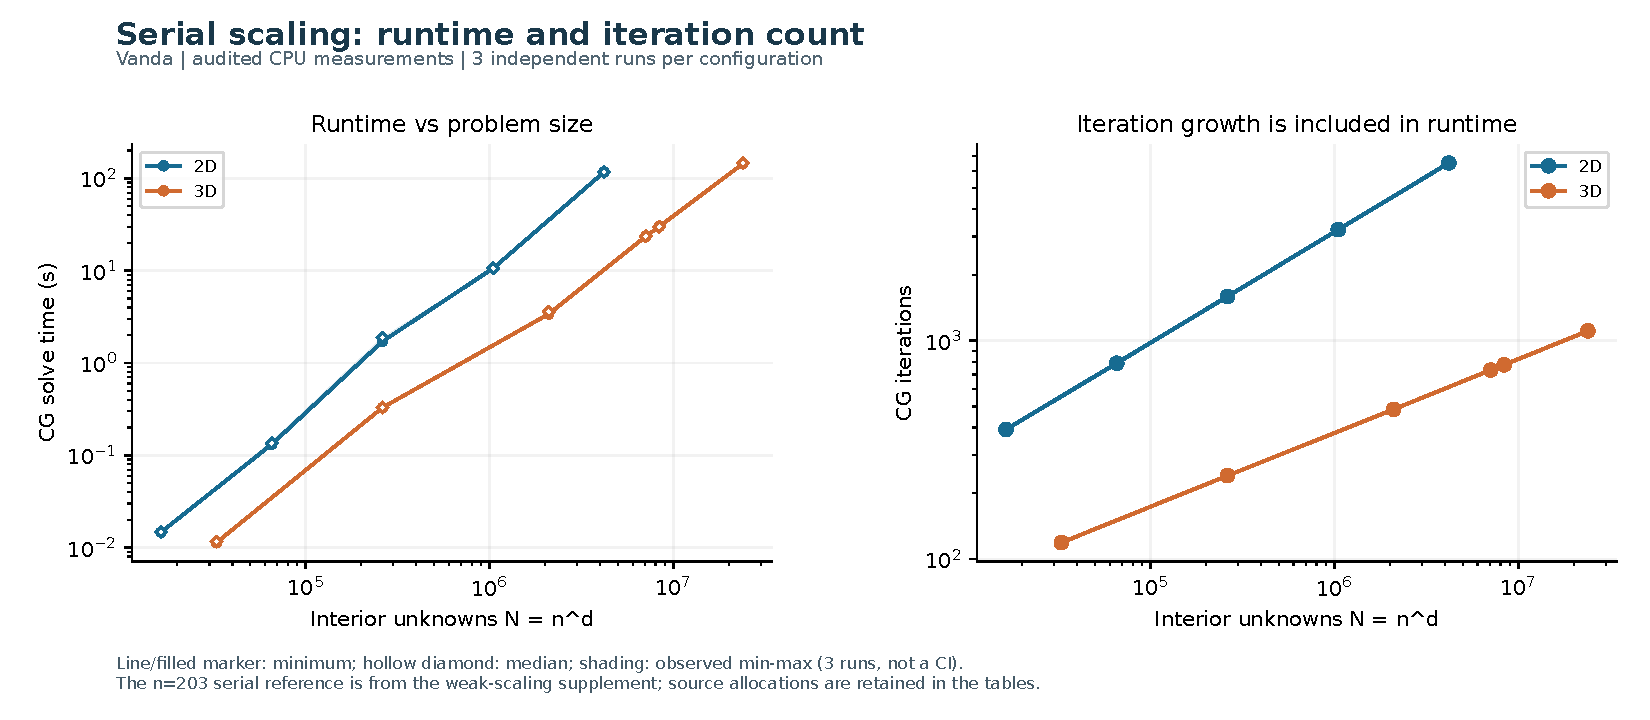
\includegraphics[width=0.9\linewidth]{serial_scaling.pdf}\\[2pt]
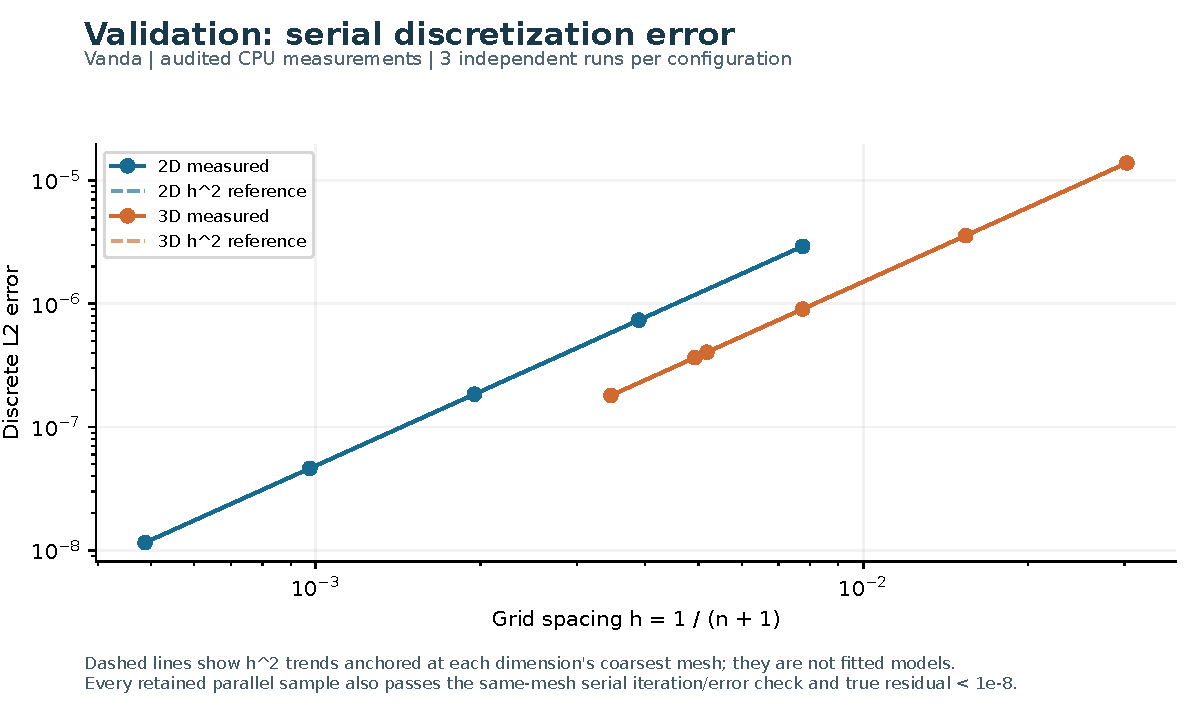
\includegraphics[width=0.9\linewidth]{serial_error.pdf}
\caption{Top: serial runtime and CG iteration count against the number of unknowns. Bottom:
discretisation error against $h$ with $h^2$ reference lines (validation of
Section~\ref{sec:validation}).}\label{fig:serial}
\end{figure}

%=====================================================================
\section{MPI performance}\label{sec:mpiresults}
%=====================================================================

\subsection{Strong scaling}
We use the largest meshes that fit our time budget: 2D $n=2048$ ($4.2\times10^6$ unknowns) and
3D $n=288$ ($2.4\times10^7$ unknowns), from 1 to 288 cores (Tables~\ref{tab:strong2d}--\ref{tab:strong3d},
Figures~\ref{fig:strong2d}--\ref{fig:strong3d}).

\begin{table}[H]
\centering\small
\caption{2D strong scaling, $n=2048$, standard CG, blocking halo. $S$ speedup, $E$ efficiency (\%);
phase times are for the Cartesian runs.}\label{tab:strong2d}
\begin{tabular}{rrrrrrrrrrr}
\toprule
& & \multicolumn{3}{c}{Cartesian} & \multicolumn{3}{c}{slab} & \multicolumn{3}{c}{Cartesian phases (s)}\\
\cmidrule(lr){3-5}\cmidrule(lr){6-8}\cmidrule(lr){9-11}
$P$ & nodes & $T$ (s) & $S$ & $E$ & $T$ (s) & $S$ & $E$ & stencil & halo & reduce\\
\midrule
\gen{strong_2d.tex}
\bottomrule
\end{tabular}
\end{table}

\begin{table}[H]
\centering\small
\caption{3D strong scaling, $n=288$, standard CG, blocking halo.}\label{tab:strong3d}
\begin{tabular}{rrrrrrrrrrr}
\toprule
& & \multicolumn{3}{c}{Cartesian} & \multicolumn{3}{c}{slab} & \multicolumn{3}{c}{Cartesian phases (s)}\\
\cmidrule(lr){3-5}\cmidrule(lr){6-8}\cmidrule(lr){9-11}
$P$ & nodes & $T$ (s) & $S$ & $E$ & $T$ (s) & $S$ & $E$ & stencil & halo & reduce\\
\midrule
\gen{strong_3d.tex}
\bottomrule
\end{tabular}
\end{table}

\begin{figure}[H]
\centering
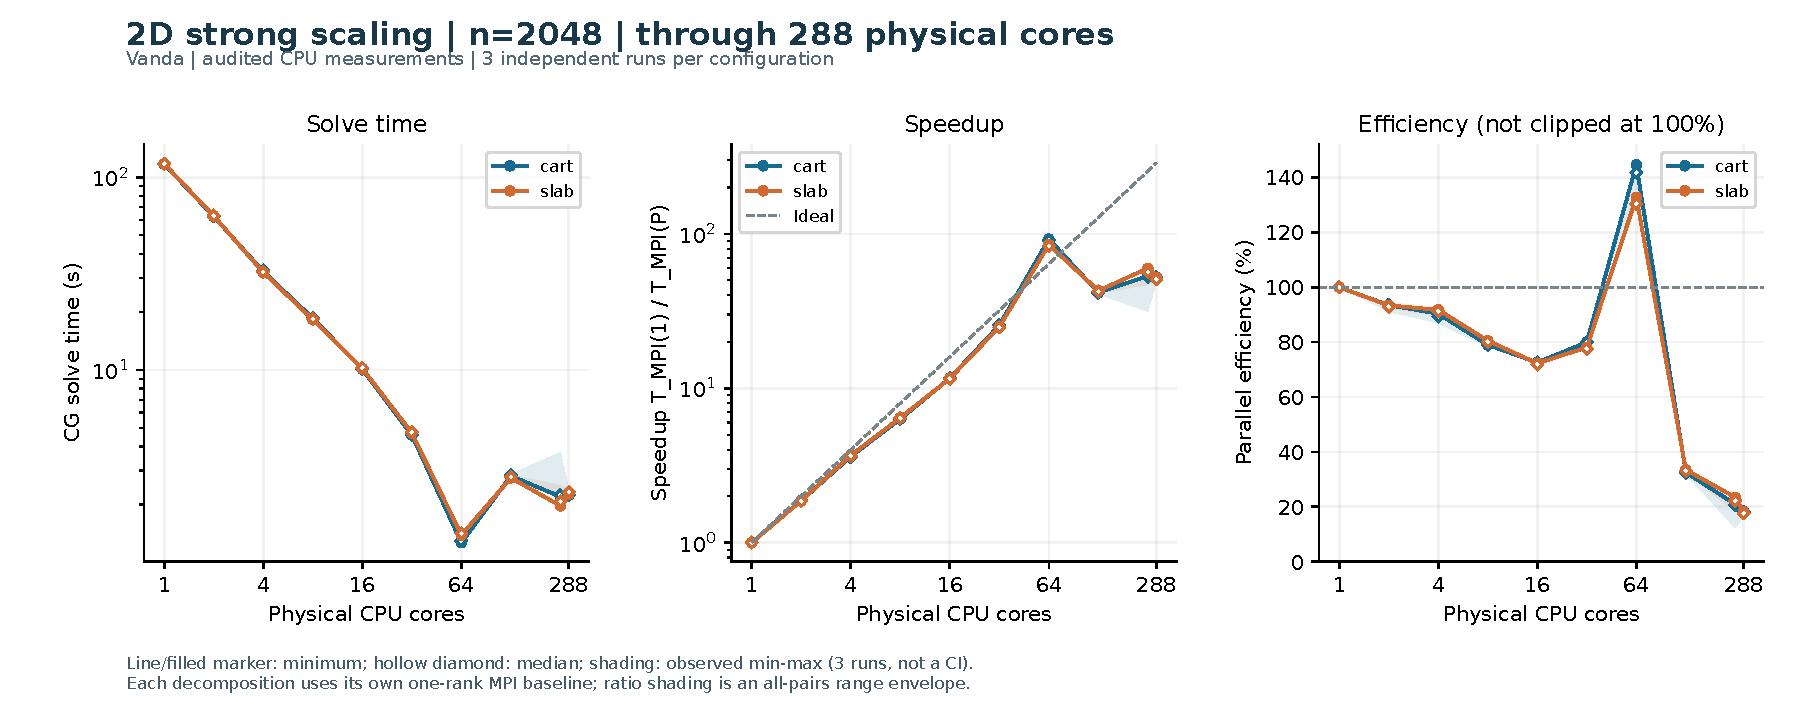
\includegraphics[width=\linewidth]{strong_2d_n2048.pdf}\\
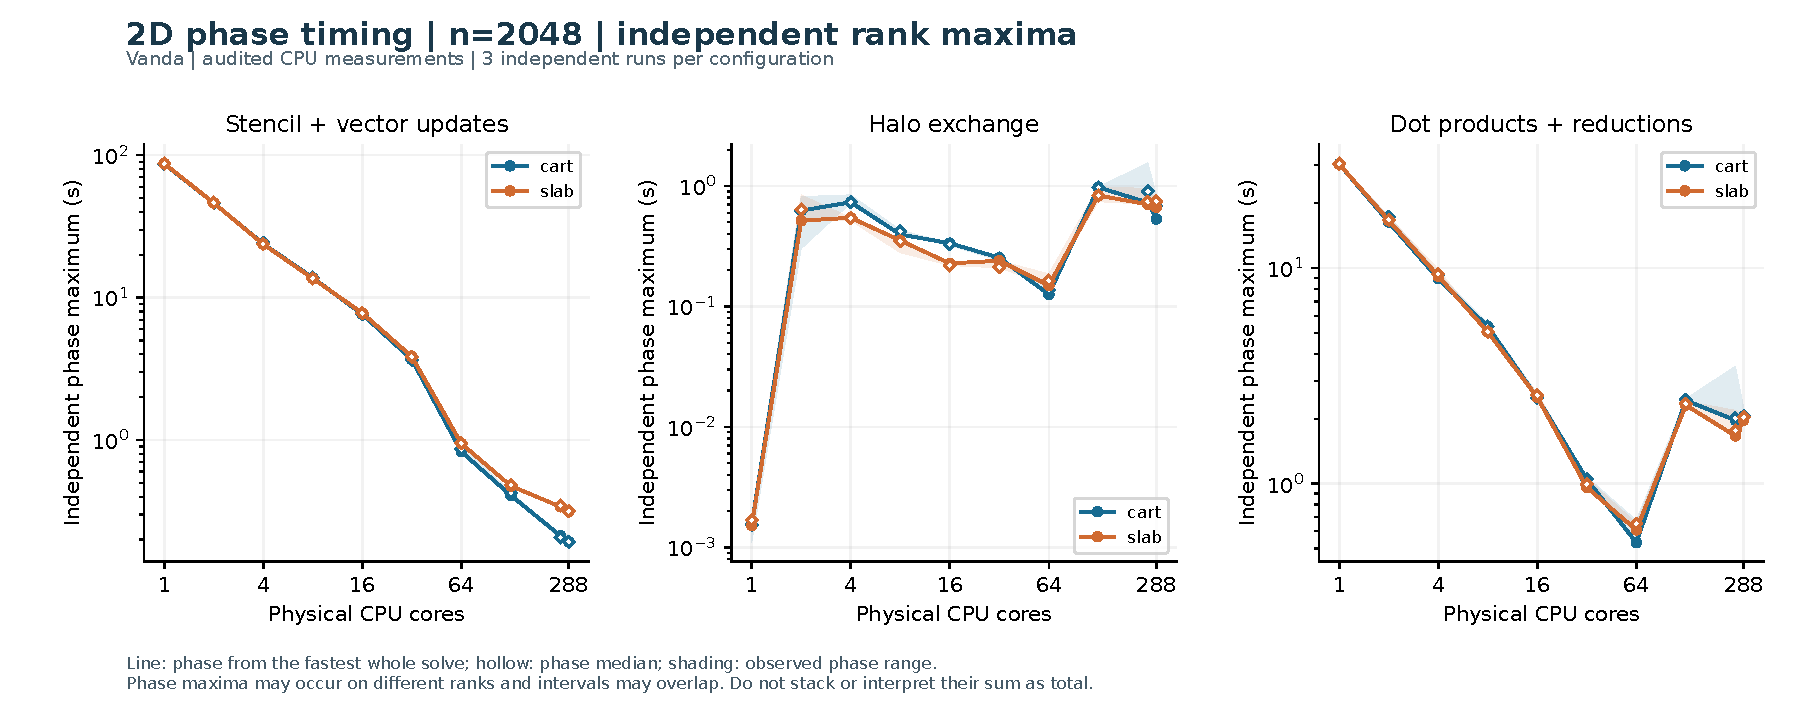
\includegraphics[width=\linewidth]{phases_2d_n2048.pdf}
\caption{2D strong scaling ($n=2048$): time, speedup and efficiency (top) and per-phase maxima
(bottom). Lines: minimum of three runs; hollow diamonds: median; shading: observed range.}\label{fig:strong2d}
\end{figure}

\begin{figure}[H]
\centering
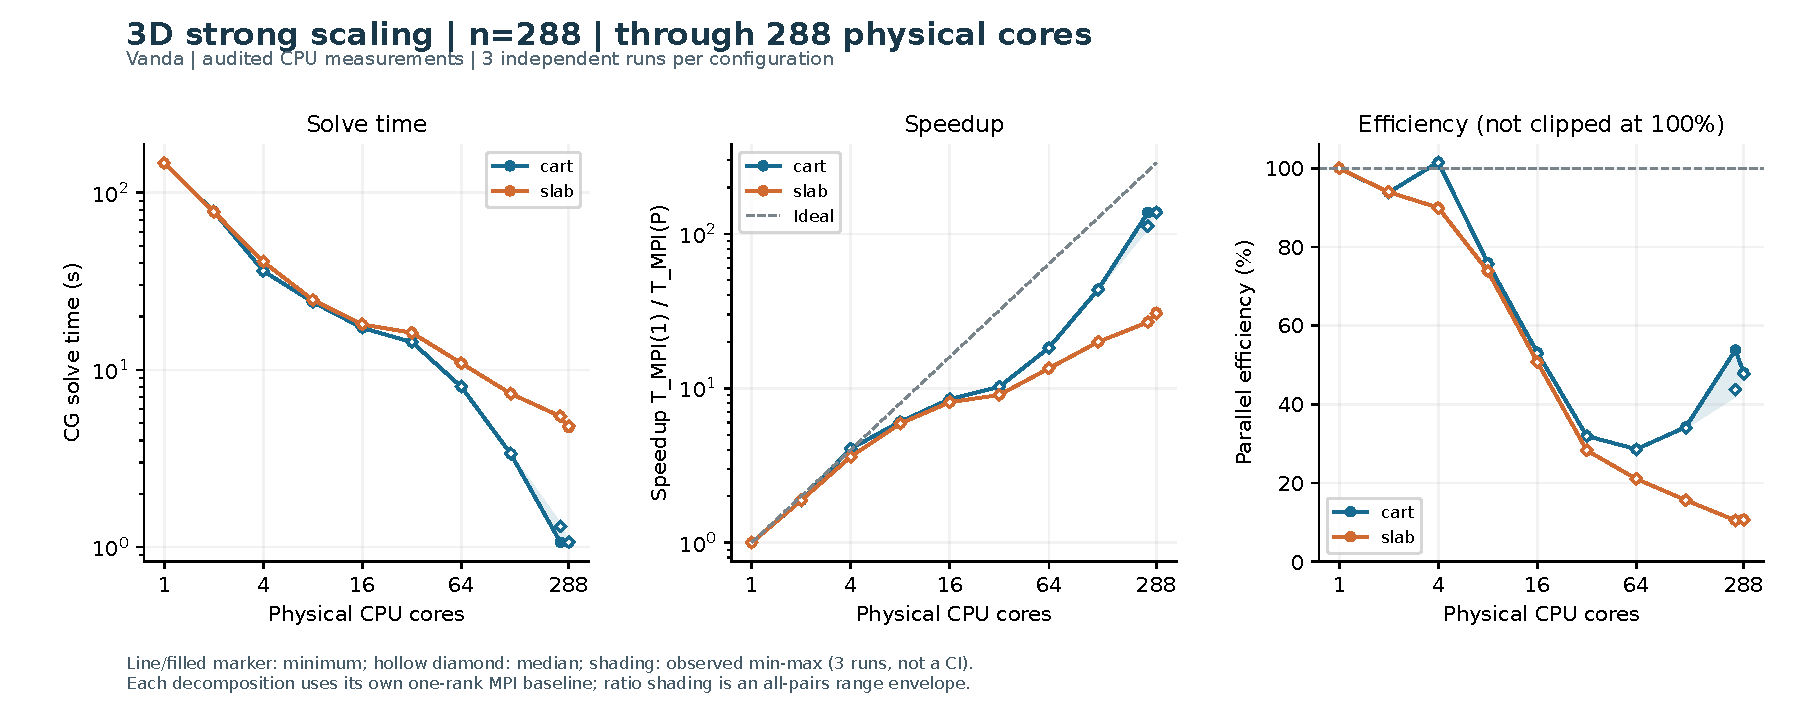
\includegraphics[width=\linewidth]{strong_3d_n288.pdf}\\
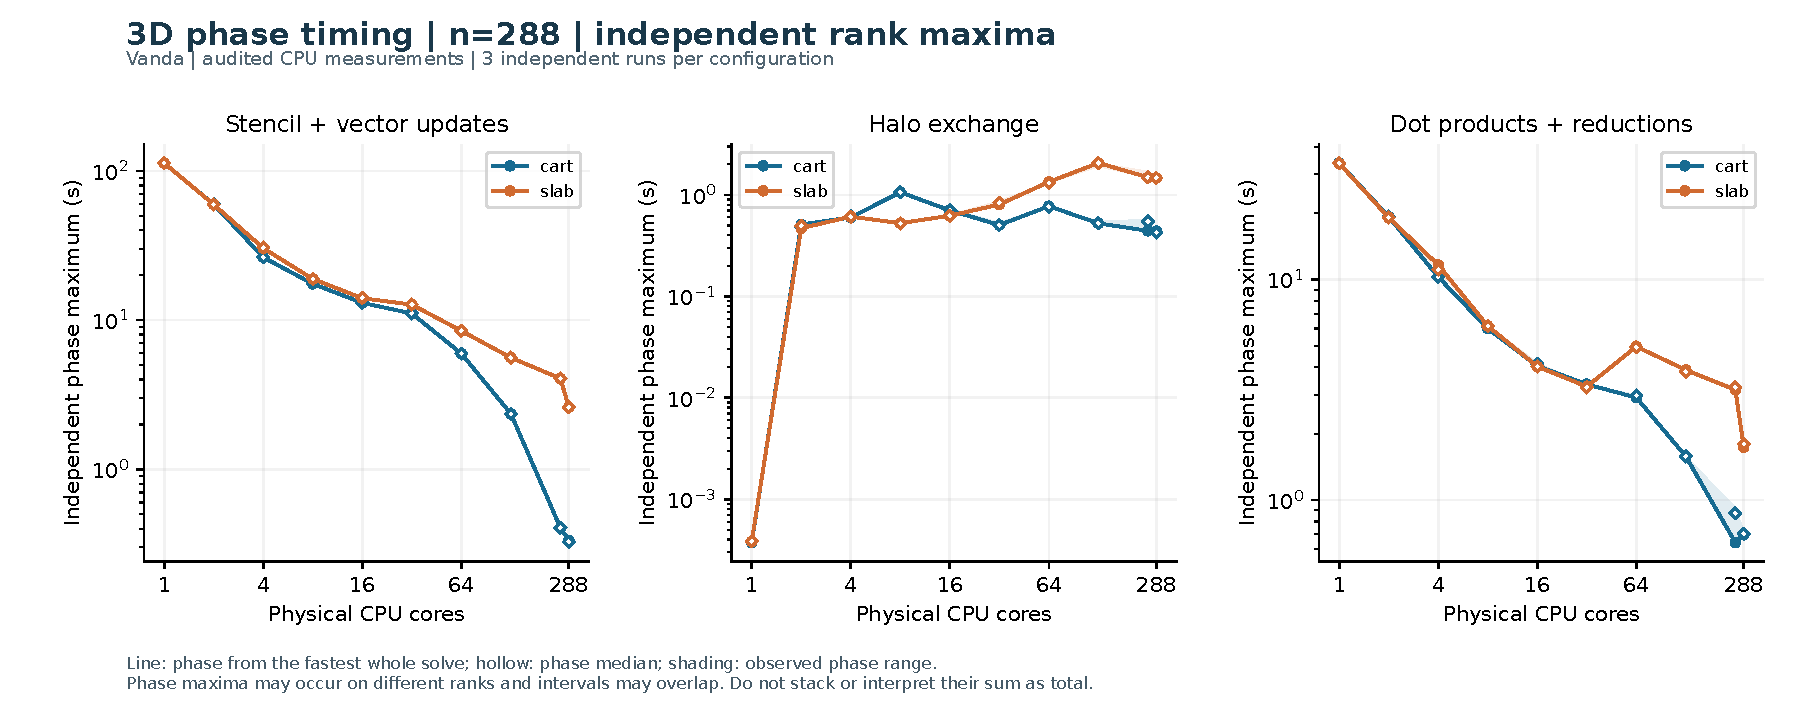
\includegraphics[width=\linewidth]{phases_3d_n288.pdf}
\caption{3D strong scaling ($n=288$) and per-phase maxima.}\label{fig:strong3d}
\end{figure}

\paragraph{Within one node (1--64 cores) the solver is limited by memory, not communication.}
Halo times stay below 1~s for all $P$, a small fraction of the total, and in 2D the efficiency
stays at 72--93\% up to 32 cores. The two meshes then behave very differently at 64 cores. The 2D
working set (five vectors of $4.2\times10^6$ doubles, $\approx170$~MB) fits in the aggregate L2 and
L3 caches of one node, so the 64-rank 2D run moves $\approx470$~MB per iteration in 0.19~ms, a rate only
caches can supply, and becomes \emph{superlinear} ($S=92.5$, $E=145\%$). The 3D working set
($\approx1$~GB) does not fit: at 64 cores the estimated traffic is $\approx400$~GB/s, which is close to
the sustainable memory bandwidth of one two-socket node, so adding cores within the node stops
helping and the 3D efficiency falls to 29\%. When the 3D problem is spread over two and then four
nodes, both the aggregate memory bandwidth and the aggregate cache grow, and the stencil time
falls from 5.96~s (64 cores) to 0.41~s (256 cores), a $14.7\times$ reduction for $4\times$ the cores.
This is why the 3D curve recovers to $S=138$ at 256 cores ($E=54\%$).

\paragraph{Across nodes the global reductions dominate.} In 2D the time \emph{increases} from 1.27~s
on one node to 2.81~s on two nodes, and stays at $\approx2.2$~s on four. The phase data show why:
the reduce time jumps from 0.53~s to 2.43~s as soon as the job spans two nodes. Dividing the reduce
time by the $2\times6512$ reductions gives the average cost of one reduction (Table~\ref{tab:reduce}):
41~$\mu$s inside a node (mostly the local dot product) but 150--190~$\mu$s once the
\texttt{Allreduce} crosses the TCP network. The 2D problem at 256 cores has only 16,384 points per
rank, so the computation per iteration (about 33~$\mu$s of stencil work) is far smaller than one
inter-node reduction; the algorithm is \emph{latency bound} and adding cores cannot help. The 3D
problem has $5.7\times$ more points and $6\times$ fewer iterations, so at 256 cores its stencil work
per iteration ($\approx370~\mu$s) still exceeds the reduction latency and the solver keeps scaling.
Within one node the reduce phase also contains waiting time: the slowest rank of each iteration
determines when the \texttt{Allreduce} completes.

\begin{table}[H]
\centering\small
\caption{Average cost of one reduction (reduce phase divided by $2\times$iterations), Cartesian,
standard CG. It includes the local dot product, the \texttt{MPI\_Allreduce} and waiting for the
slowest rank.}\label{tab:reduce}
\begin{tabular}{lrrr}
\toprule
dim & $P$ & nodes & $\mu$s per reduction\\
\midrule
\gen{reduce.tex}
\bottomrule
\end{tabular}
\end{table}

\paragraph{Decomposition.} In 2D slab and Cartesian decompositions perform alike (their halo volumes
of 32~KiB and 4--8~KiB per iteration are both negligible beside the reductions). In 3D the Cartesian
decomposition is $5.1\times$ faster at 256 cores (1.06~s against 5.46~s): a 3D slab face is a full
$288\times288$ plane, and with 256 or 288 slabs each rank owns only one or two planes, so it sends as
many values as it owns (Table~\ref{tab:comm}) and its stencil is applied to blocks that are too thin
to vectorise or reuse cache well. Cartesian decomposition is the only choice that scales in 3D.

\subsection{Weak scaling}
For weak scaling the mesh grows with $P$ so that the number of unknowns per core is constant:
$n=128\sqrt P$ in 2D (16,384 points per core) and $n=\mathrm{round}(32\sqrt[3]{P})$ in 3D
(32,768 per core; $-0.3\%$ at $P=256$ due to rounding), up to 256 cores (Table~\ref{tab:weak},
Figure~\ref{fig:weak}).

\begin{table}[H]
\centering\small
\caption{Weak scaling (Cartesian, standard CG). $E_w=T(1)/T(P)$ for the whole solve;
$E_{\text{it}}$ uses the time per iteration.}\label{tab:weak}
\begin{tabular}{lrrrrrrrrr}
\toprule
dim & $P$ & $n$ & $N/P$ & iters & $T$ min (s) & $T$ median (s) & $\mu$s/it & $E_w$ (\%) & $E_{\text{it}}$ (\%)\\
\midrule
\gen{weak.tex}
\bottomrule
\end{tabular}
\end{table}

\begin{figure}[H]
\centering
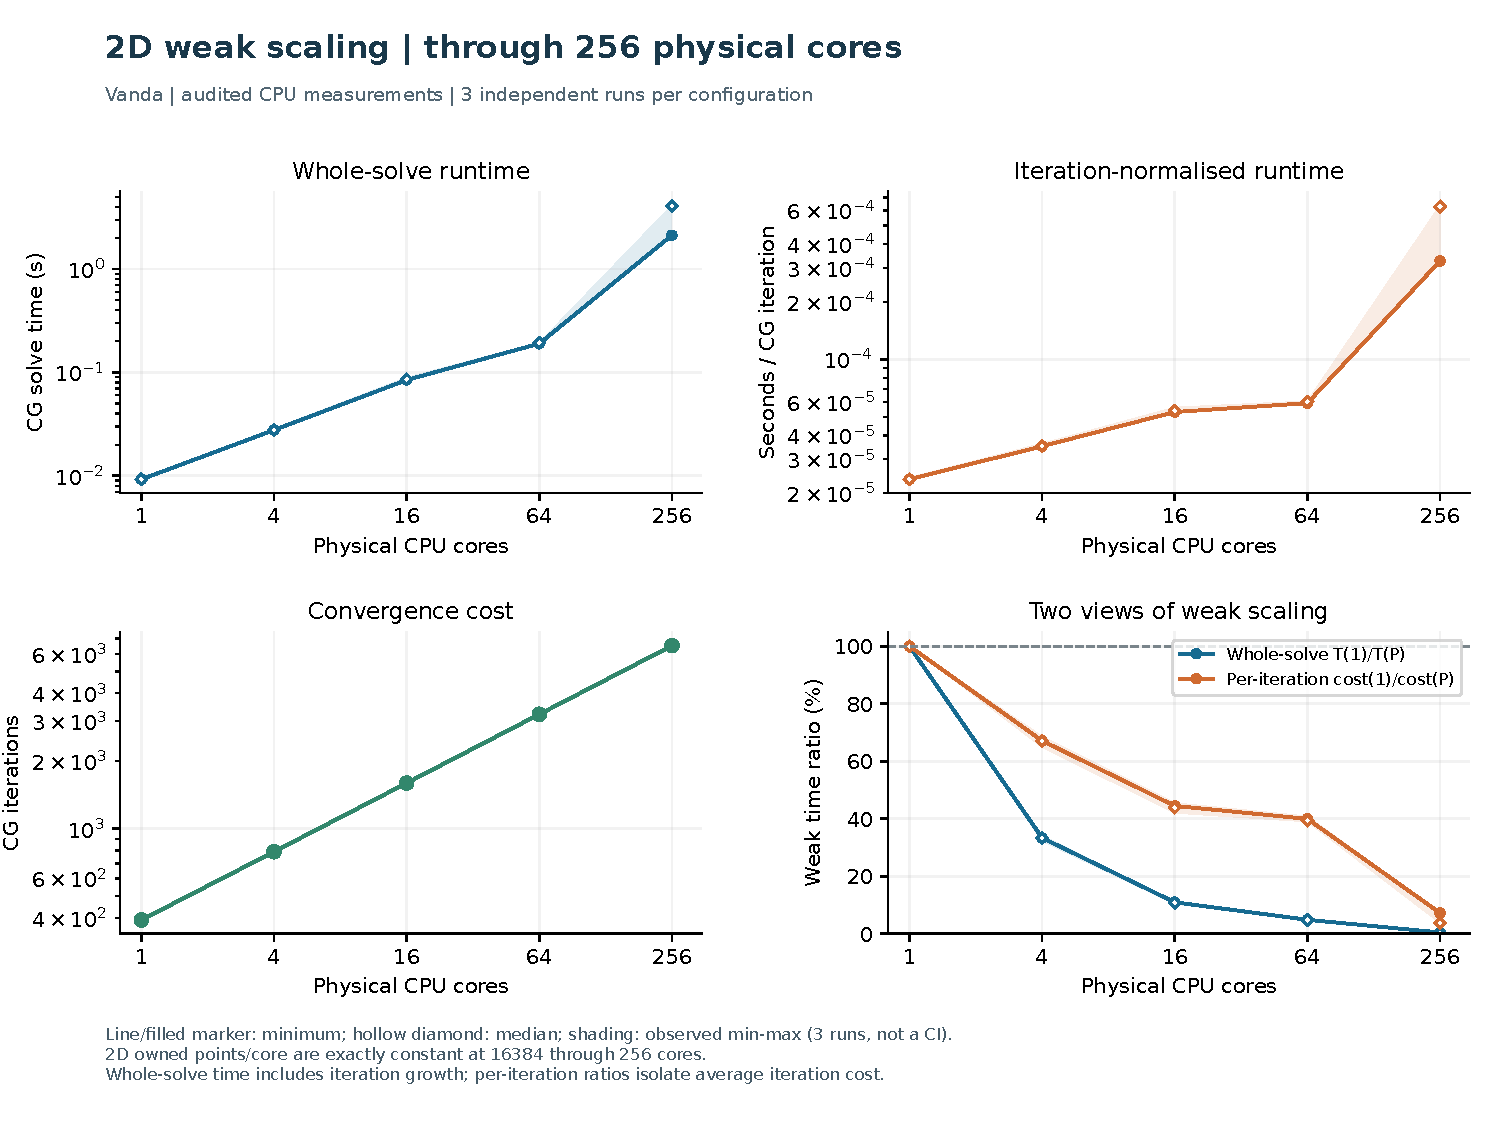
\includegraphics[width=0.8\linewidth]{weak_2d.pdf}\\
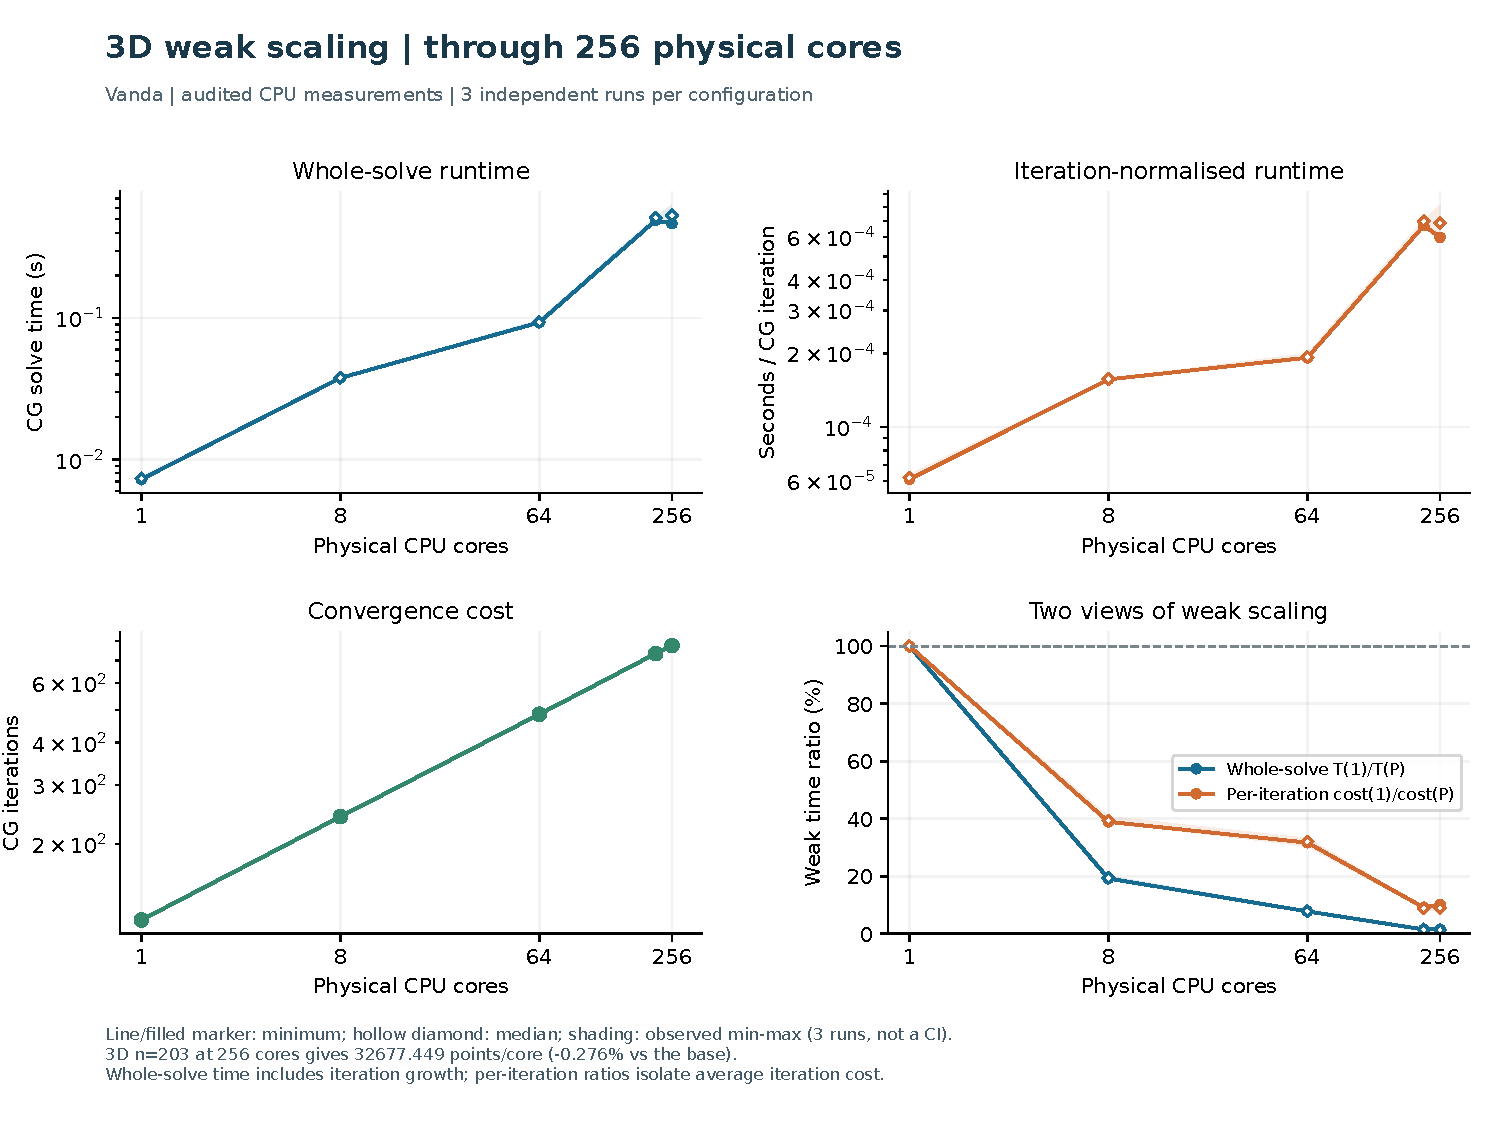
\includegraphics[width=0.8\linewidth]{weak_3d.pdf}
\caption{Weak scaling in 2D (top) and 3D (bottom): whole-solve and per-iteration time, weak
efficiency, and iteration growth.}\label{fig:weak}
\end{figure}

Whole-solve weak efficiency necessarily decays for unpreconditioned CG, because the iteration
count grows with $n$ (392 to 6512 in 2D, 119 to 775 in 3D) even though the work per iteration
per core is constant. The per-iteration efficiency $E_{\text{it}}$ removes this algorithmic
effect and isolates the parallel overhead. It falls to 40\% (2D) and 32\% (3D) at 64 cores on one
node, where 64 ranks share the memory bandwidth that a single rank had alone, and then to 7--10\%
at 216--256 cores on several nodes, where each iteration pays two inter-node reductions: at 2D
$P=256$, 291~$\mu$s of the 327~$\mu$s per iteration is reduce time. The 2D endpoint is also the
noisiest point of the study (median $1.9\times$ the minimum), as expected for a run dominated by network
latency.

\subsection{Communication-reducing variants}
Table~\ref{tab:variants} and Figure~\ref{fig:variants} compare the four combinations of halo
mode and CG variant at 64 cores (one node) and 256 cores (four nodes).

\begin{table}[H]
\centering\small
\caption{Solve time (s) for the four halo/CG choices (Cartesian; best per row in bold), and reduce
phase of the blocking runs.}\label{tab:variants}
\begin{tabular}{lrrrrrrr}
\toprule
& & \multicolumn{4}{c}{total time (s)} & \multicolumn{2}{c}{reduce phase (s)}\\
\cmidrule(lr){3-6}\cmidrule(lr){7-8}
dim & $P$ & block/std & overlap/std & block/pipe & overlap/pipe & std & pipe\\
\midrule
\gen{variants.tex}
\bottomrule
\end{tabular}
\end{table}

\begin{figure}[H]
\centering
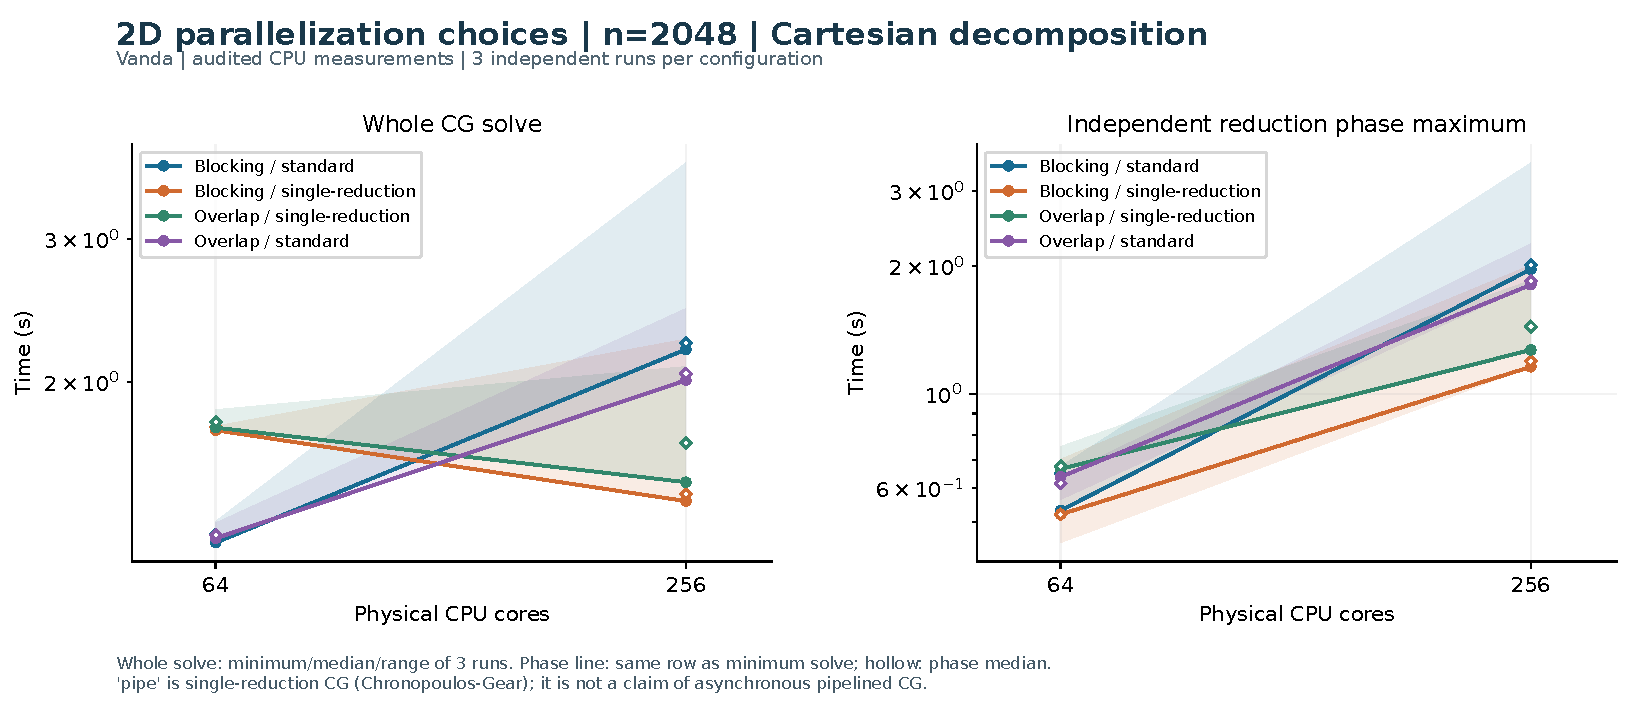
\includegraphics[width=0.92\linewidth]{variants_2d_n2048.pdf}\\[2pt]
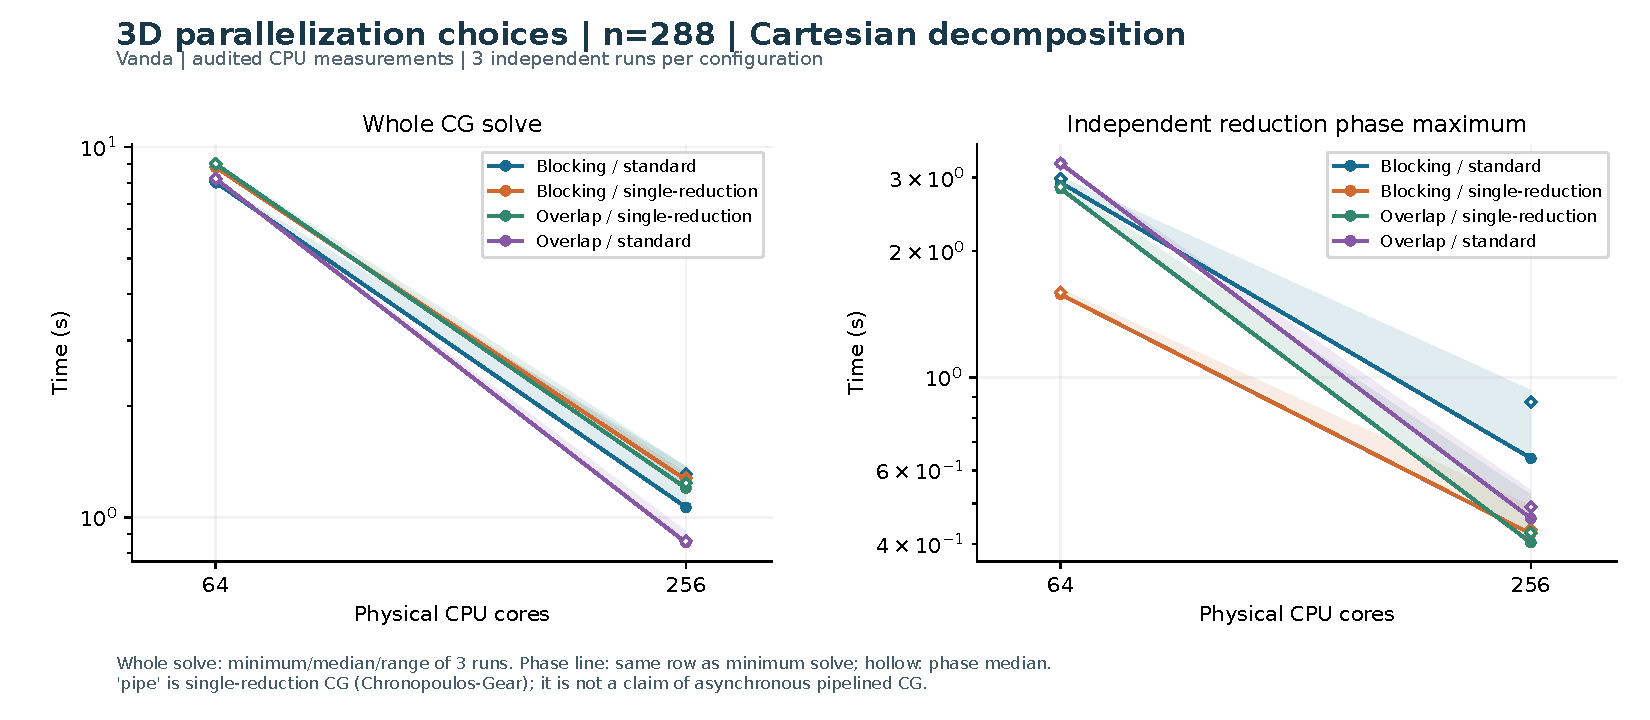
\includegraphics[width=0.92\linewidth]{variants_3d_n288.pdf}
\caption{Halo mode and CG variant at 64 and 256 cores, 2D (top) and 3D (bottom).}\label{fig:variants}
\end{figure}

The single-reduction CG addresses exactly the bottleneck identified above. In the latency-bound
2D case at 256 cores it reduces the reduce phase from 1.97~s to 1.16~s and the total time by 35\%
(2.19~s to 1.42~s). Where the solver is still bandwidth bound (64 cores in both dimensions, and 3D
at 256 cores) its two extra vector updates cost more than the saved reduction, and it is 6--38\%
slower. Overlapping the halo with interior computation helps when the halo is significant and
there is enough interior work to hide it: 3D at 256 cores runs 20\% faster (0.85~s against 1.06~s;
halo phase 0.18~s against 0.44~s). It does not help in 2D, where the halo is small. There is therefore no
universally best variant: the right choice depends on whether bandwidth, neighbour messages or
global latency dominates, which is precisely what the phase breakdown measures.

%=====================================================================
\section{MPI+X performance}\label{sec:mpix}
%=====================================================================

\subsection{MPI+OpenMP at a fixed number of cores}
We use all 288 cores of four nodes and vary the split between MPI ranks and OpenMP threads per
rank, from $288\times1$ to $4\times72$ (one rank per socket would be $8\times36$; $4\times72$ is one
rank per node). Table~\ref{tab:hybrid} and Figure~\ref{fig:hybrid} give the results relative to
pure MPI with 288 ranks.

\begin{table}[H]
\centering\small
\caption{Fixed 288 cores: MPI ranks $\times$ OpenMP threads. Ratio $=T/T_{\text{pure MPI}}$
(larger is slower).}\label{tab:hybrid}
\begin{tabular}{lrrrrrr}
\toprule
& & & \multicolumn{2}{c}{2D, $n=2048$} & \multicolumn{2}{c}{3D, $n=288$}\\
\cmidrule(lr){4-5}\cmidrule(lr){6-7}
version & ranks & threads & $T$ (s) & ratio & $T$ (s) & ratio\\
\midrule
\gen{hybrid.tex}
\bottomrule
\end{tabular}
\end{table}

\begin{figure}[H]
\centering
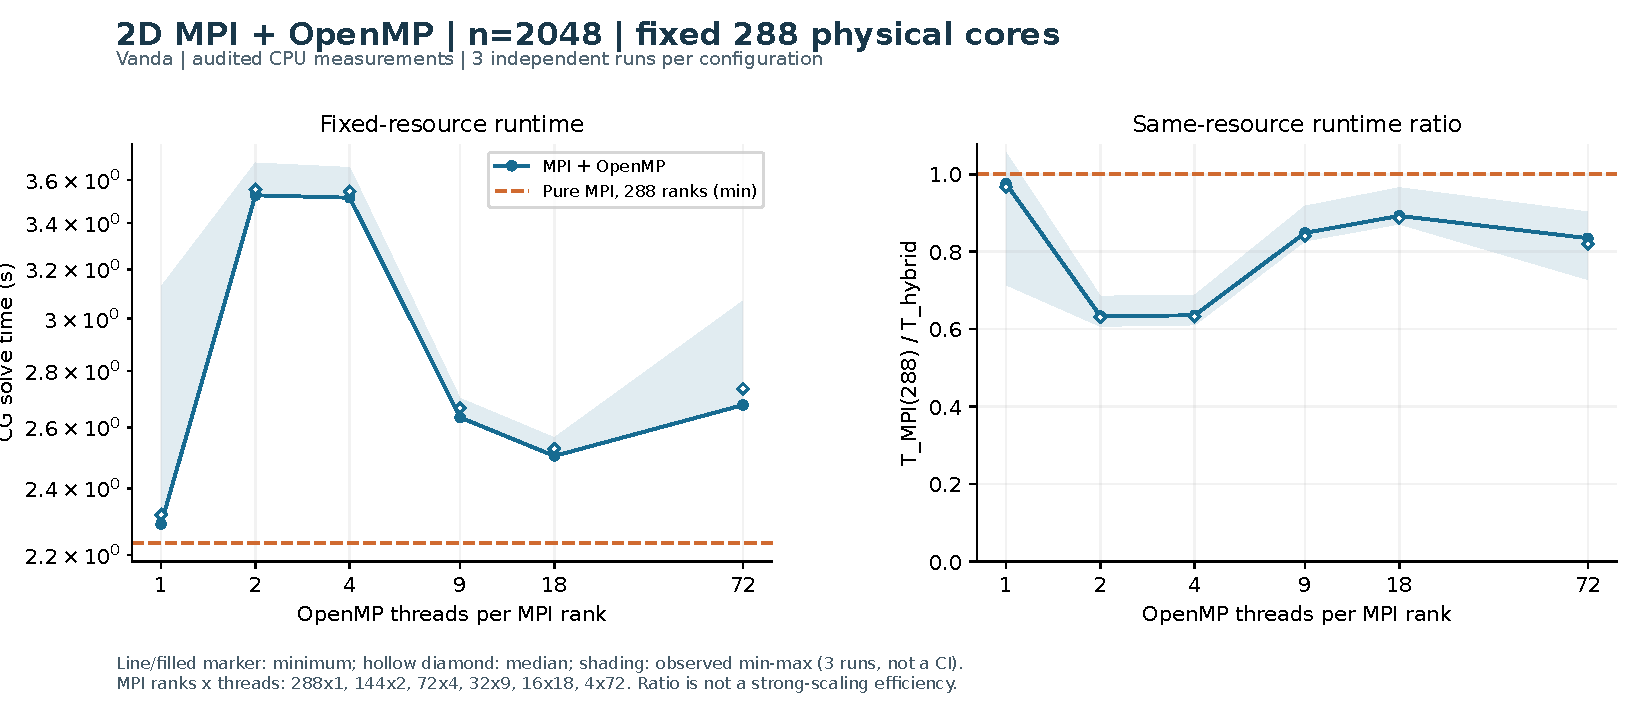
\includegraphics[width=0.92\linewidth]{hybrid_2d_n2048.pdf}\\[2pt]
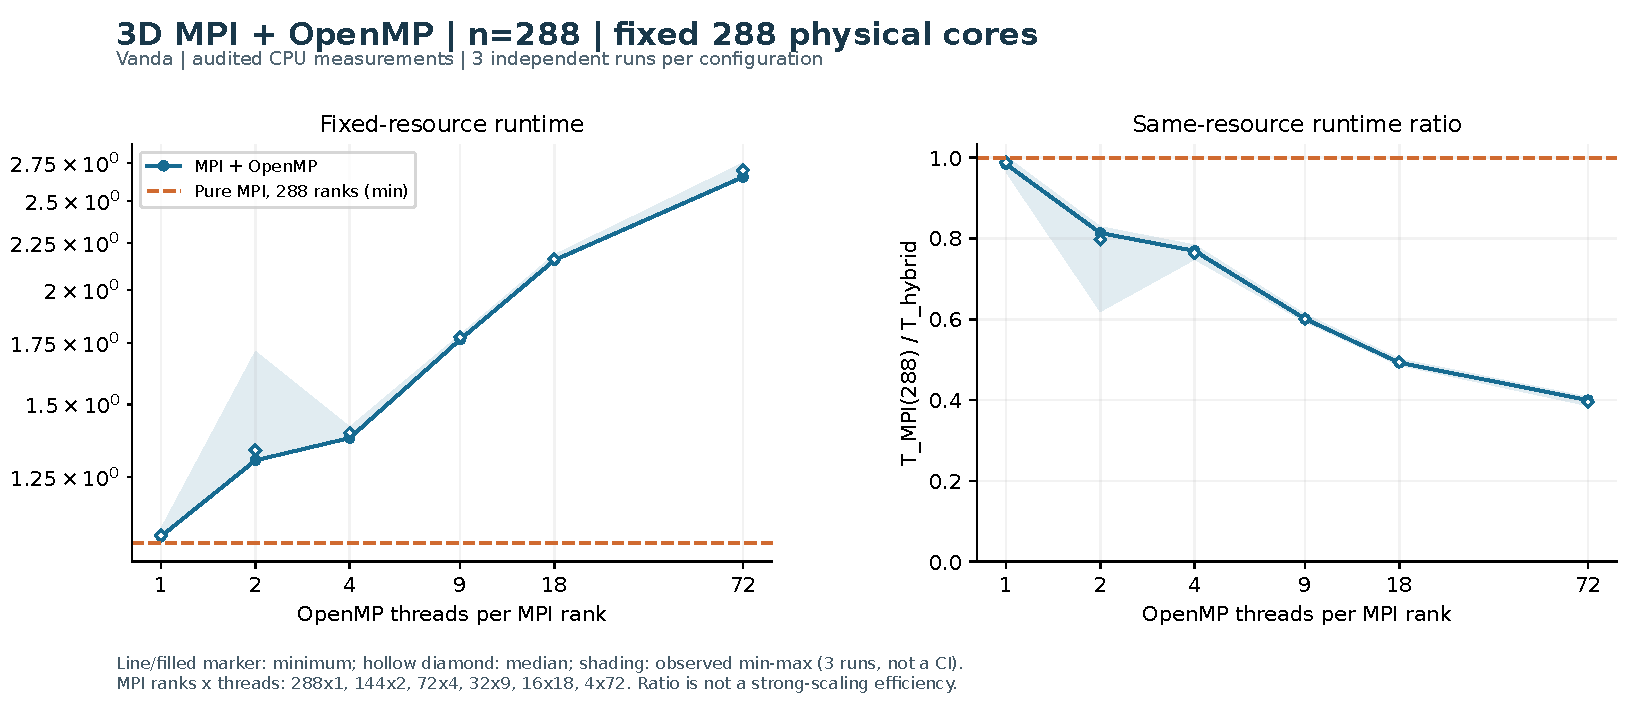
\includegraphics[width=0.92\linewidth]{hybrid_3d_n288.pdf}
\caption{MPI ranks $\times$ OpenMP threads on 288 cores, 2D (top) and 3D (bottom).}\label{fig:hybrid}
\end{figure}

\begin{table}[H]
\centering\small
\caption{Phase maxima (s) of the hybrid runs.}\label{tab:hybridphases}
\begin{tabular}{llrrr}
\toprule
dim & ranks$\times$threads & stencil & halo & reduce\\
\midrule
\gen{hybrid_phases.tex}
\bottomrule
\end{tabular}
\end{table}

With one thread per rank the hybrid solver matches pure MPI to within 2\%, so the threading
layer itself costs little. Adding threads did not make the solver faster for these meshes; the
best multi-threaded splits were $16\times18$ in 2D (12\% slower than pure MPI) and $144\times2$ in
3D (23\% slower). The phase breakdown (Table~\ref{tab:hybridphases}) shows three competing effects.
\begin{itemize}
\item \emph{Fewer ranks in each reduction.} In 2D the reduce phase drops from 2.09~s ($288\times1$) to
1.15~s ($4\times72$), confirming that hybrid parallelism lowers global-reduction cost. With
$144\times2$ and $72\times4$, however, it rises to $\approx3.1$~s; these splits leave ranks of a
node spread over both sockets with small thread teams, and the extra fork--join and imbalance
appears as waiting time in the reductions.
\item \emph{Funnelled communication.} Halo time grows monotonically with the thread count (3D: 0.43~s
to 1.67~s). Fewer, larger blocks have larger faces, and with \texttt{MPI\_THREAD\_FUNNELED} the
master thread alone packs and sends them while the other threads wait.
\item \emph{NUMA.} With 72 threads per rank the stencil time more than doubles (2D: 0.20~s to 0.66~s).
Vectors are zero-initialised by the master thread, so by the first-touch page placement policy
all of a rank's memory resides on one socket and half of its threads read remote memory.
Parallel first-touch initialisation would remove this effect.
\end{itemize}
In 3D, where reductions matter less, the loss of halo efficiency dominates and every
multi-threaded split is slower. In 2D, the reduction saving and the halo/NUMA costs nearly cancel.

\subsection{MPI+CUDA on GPUs}
Table~\ref{tab:gpu} and Figure~\ref{fig:gpu} show the CUDA solver on one and two NVIDIA A40 GPUs (one
per node), with both halo transports. The 3D GPU mesh is $n=256$ ($1.7\times10^7$ unknowns), the largest
whose serial reference fits the time budget; the last column compares with the serial CPU solver on
the same mesh.

\begin{table}[H]
\centering\small
\caption{MPI+CUDA strong scaling on A40 GPUs. $S$ and $E$ (\%) are relative to one GPU with the same transport;
``vs serial'' is the speedup over one CPU core on the same mesh.}\label{tab:gpu}
\begin{tabular}{llrrrrrrrr}
\toprule
mesh & transport & GPUs & $T$ (s) & $S$ & $E$ & stencil & halo & reduce & vs serial\\
\midrule
\gen{gpu.tex}
\bottomrule
\end{tabular}
\end{table}

\begin{figure}[H]
\centering
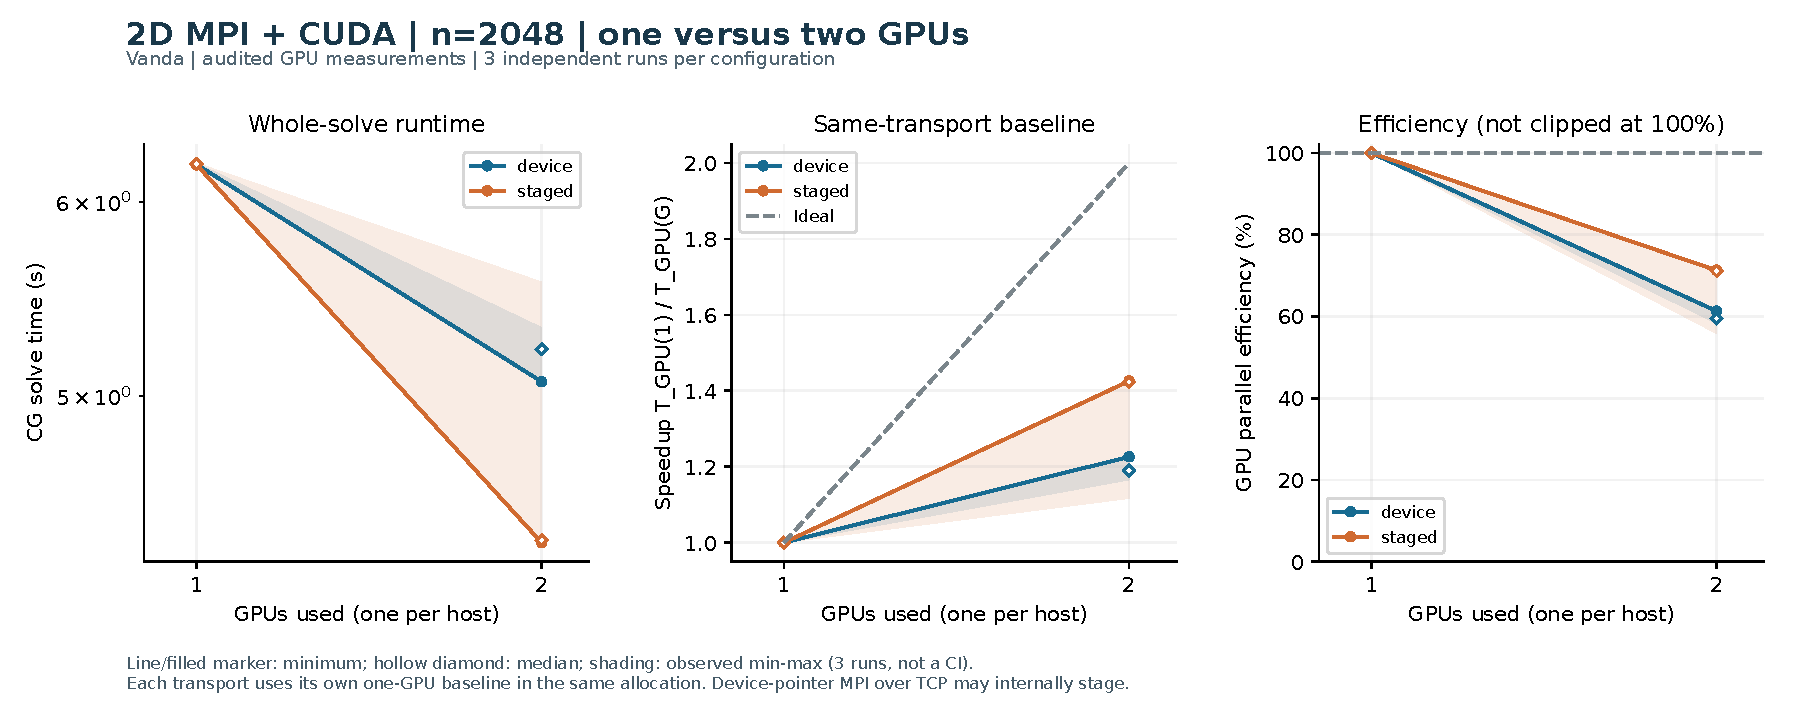
\includegraphics[width=0.92\linewidth]{gpu_2d_n2048.pdf}\\[2pt]
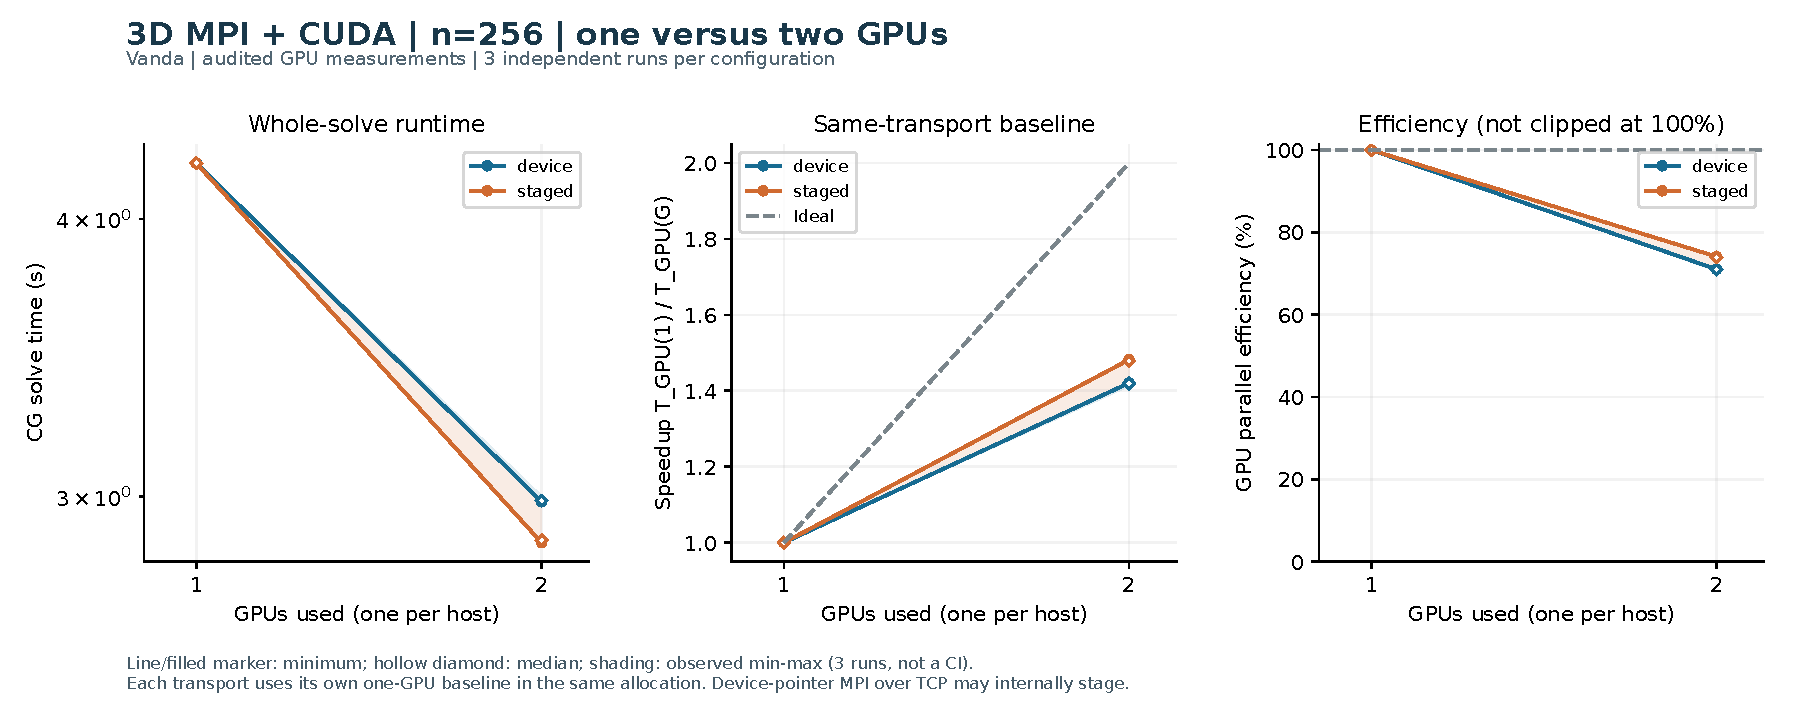
\includegraphics[width=0.92\linewidth]{gpu_3d_n256.pdf}
\caption{MPI+CUDA on one and two A40 GPUs, 2D (top) and 3D (bottom), staged and device transports.}\label{fig:gpu}
\end{figure}

One A40 solves the problems $18.5\times$ (2D) and $18.9\times$ (3D) faster than one CPU core, roughly
the performance of 16--32 cores of one node. As on the CPU, the GPU solver is memory-bandwidth
bound: with $\approx112$ bytes per unknown per iteration, the single-GPU runs sustain about 490~GB/s
(2D) and 440~GB/s (3D), 60--70\% of the A40's 696~GB/s peak; the A40's low double-precision
arithmetic rate is therefore not the limit. The reduce phase is substantial even on one GPU
(1.59~s in 2D, i.e.\ 120~$\mu$s per dot product): each reduction launches two kernels and copies a
scalar back to the host, which synchronises the device. A fused single-reduction CG would help
the GPU at least as much as the CPU.

With two GPUs on two nodes the stencil time halves exactly (2D: 4.63~s to 2.30~s), but each
iteration now pays a halo exchange between nodes (0.73--1.52~s) and inter-node reductions, so the
speedup is 1.23--1.48 (efficiency 61--74\%). The staged transport was faster than device-pointer
transport in both meshes. Since inter-node traffic used TCP, CUDA-aware MPI cannot transfer
directly from GPU memory to the network and must stage the data internally, with its own
synchronisation; explicit staging in our code is at least as efficient. The site limited jobs
to two GPUs, so we could not measure beyond two devices.

%=====================================================================
\section{Overall discussion}\label{sec:discussion}
%=====================================================================

\paragraph{How the problem was parallelised.} Parallelism comes from the data: the grid is
split into blocks, and each operation of an iteration is parallelised with the cheapest technique
for its data dependencies (Table~\ref{tab:techniques}). Vector updates are purely local. The
stencil needs only nearest-neighbour data, handled by halo exchange between MPI ranks and by
shared memory between threads and GPU threads. The dot products need data from every process and
are the only global operation. The design decisions that mattered most in our measurements were:
(i) Cartesian rather than slab decomposition in 3D ($5\times$); (ii) reducing the number of global
reductions when they dominate ($35\%$ at 256 cores in 2D); (iii) overlapping halo exchange with
interior work when halos are large ($20\%$ in 3D at 256 cores); and (iv) using one MPI rank per
core rather than wide OpenMP teams, unless reduction latency is the main cost.

\paragraph{Which parts need the most communication.} By volume, the halo exchange: tens to
hundreds of KiB per rank per iteration, against 8--16 bytes for a reduction. By cost, the global
reductions: they move almost no data, but they are latency bound, grow with $\log P$ and the
number of nodes, and force all ranks to synchronise twice per iteration. The halo is a surface
term that shrinks as $P$ grows (as $(N/P)^{(d-1)/d}$ for Cartesian blocks), whereas the reduction
cost does not shrink at all. This is why 3D, with more work per point of surface and fewer
iterations, scales to 256 cores while 2D stops at one node; and why the communication-avoiding
variants that matter are those that reduce the \emph{number} of global synchronisations rather
than the message volume.

\paragraph{Memory hierarchy.} Both CPU and GPU versions are memory-bandwidth bound. This explains
the superlinear 2D speedup at 64 cores (the working set fits in cache), the efficiency loss when a
single node fills up, the recovery of the 3D solver across nodes, and the $\approx19\times$ GPU
advantage, which is close to the ratio of GPU to single-core memory bandwidth.

\paragraph{Limitations.} Inter-node communication used TCP, not RDMA, which makes reduction
latency higher than on a tuned InfiniBand stack; the conclusions about where the cross-over from
bandwidth-bound to latency-bound happens depend on this. Each configuration was run three
times, so variability (up to 27\% coefficient of variation at the 2D 256-core points) limits fine
comparisons. GPU runs were limited to two devices. We did not use a preconditioner; a multigrid
or block-Jacobi preconditioner would reduce the iteration count and therefore the number of
reductions, at the cost of more communication per iteration.

%=====================================================================
\section{Conclusion}\label{sec:conclusion}
%=====================================================================
We implemented a matrix-free CG solver for the 2D and 3D Poisson equation in serial, MPI,
MPI+OpenMP and MPI+CUDA versions that share one algorithm and agree with each other to rounding
error, and we validated second-order accuracy against a manufactured solution. Serial CG is
memory-bandwidth bound and its cost grows like $N^{3/2}$ (2D) and $N^{4/3}$ (3D), slightly faster
in practice once the working set leaves the cache. Pure MPI scales to 256 cores with $138\times$
speedup for the 3D problem with Cartesian decomposition, while the 2D problem becomes bound by
global-reduction latency once it spans more than one node; the single-reduction CG variant
recovers 35\% of that loss. At a fixed core count, hybrid MPI+OpenMP reduces the cost of the
global reductions but did not outperform pure MPI because of funnelled communication and NUMA
effects. One A40 GPU replaces about 16--32 CPU cores, and two GPUs give a $1.4$--$1.5\times$ speedup
limited by inter-node halo and reduction latency.

\paragraph{Use of AI.} Generative AI tools (Anthropic Claude and OpenAI Codex) were used to assist
in drafting code, tests, job scripts and this report; all output was reviewed, tested and
validated by the authors, who take full responsibility for the content.

\paragraph{Code.} The source code, build instructions and the scripts that reproduce every table
and figure are at \url{https://github.com/ZYKuni/NUS_DSA5208_project3_1107} (see \texttt{README.md}).

\begin{thebibliography}{9}\small
\bibitem{hestenes1952} M.~R. Hestenes and E.~Stiefel. Methods of conjugate gradients for solving linear systems.
\emph{Journal of Research of the National Bureau of Standards}, 49(6):409--436, 1952.
\bibitem{chronopoulos1989} A.~T. Chronopoulos and C.~W. Gear. $s$-step iterative methods for symmetric linear systems.
\emph{Journal of Computational and Applied Mathematics}, 25(2):153--168, 1989.
\bibitem{saad2003} Y.~Saad. \emph{Iterative Methods for Sparse Linear Systems}, 2nd ed. SIAM, 2003.
\bibitem{mpi41} Message Passing Interface Forum. \emph{MPI: A Message-Passing Interface Standard, Version 4.1}, 2023.
\bibitem{openmp52} OpenMP Architecture Review Board. \emph{OpenMP Application Programming Interface, Version 5.2}, 2021.
\end{thebibliography}

\end{document}
